\documentclass{article}
\usepackage{graphicx}
\usepackage{amsmath}
\usepackage{float}
\usepackage{textgreek}
\usepackage{siunitx}
\usepackage{subcaption}


\title{PHY 338k Lab Report 1}
\author{Lily Nguyen with Anna Grove}
\date{September 18, 2025}

\begin{document}

\maketitle

\section{Introduction}


\section{Lab 1: Basic measurements and oscilloscope use}

\subsection{Wiring inside the breadboard}

Using a digital multimeter in continuity mode, we tested the internal
connections of the breadboard. Figure~\ref{fig:breadboard} shows a diagram
of the wiring.

\begin{figure}[h!]
    \centering
    \includegraphics[width=0.4\textwidth]{1.1a.png}
    \caption{Schematic of the internal wiring of the breadboard.}
    \label{fig:breadboard}
\end{figure}

\subsection{Output impedance}

\subsubsection{Open circuit voltage}

With the circuit setup as in Figure 1-7, we set $V_\text{in}=+5\si{\volt}$ and
measured the open circuit output voltage. Using the DMM in DC mode, we got 
$V_\text{open}=6.42\si{\volt}$.

\subsubsection{Closed circuit current}

With the circuit set up as in Figure 1-8, we measured the short circuit output
current by placing the DMM in series between $V_\text{out}$ and GND. We measured
the short current as $I_\text{short}=0.61\si{\milli\ampere}$.

\subsubsection{Output impedance}

Using our measured open circuit voltage short circuit current, we calculated
the output impedance of the circuit as:

\begin{equation}
    Z_\text{out}=\frac{V_\text{open}}{I_\text{short}}\approx10.5\si{\kilo\ohm}.
\end{equation}

\noindent This value is consistent with the resistance from the circuit setup. For
resistor-only circuits, the output impedance is just the total resistance value.


\subsection{Voltage divider}

\subsubsection{Voltage divider circuit}

Next, we constructed the voltage divider circuit shown in Figure 1-9 using 
$V_\text{in}=+5\si{\volt}$. Using the voltage divider formula, we calculated:

\begin{equation}
    V_\text{out}=V_\text{in}\frac{R_2}{R+1+R_2}=5\cdot\frac{9.93\si{\ohm}}{9.93\si{\ohm}+9.93\si{\ohm}}=2.50\si{\volt}.
\end{equation}

\noindent Our measured value for $V_\text{out}$ was $3.207\si{\volt}$. While it differs
from the theoretical prediction by about $0.71\si{\volt}$, it is within the correct
order of magnitude, and the discrepancy is likely due to experimental error or limitations
in the resistor tolerance.

\subsubsection{General case voltage divider}

For the general case, the voltage divider output is given by:

\begin{equation}
    V_\text{out}=V_\text{in}\frac{R_2}{R_1+R_2}.
\end{equation}

\noindent In the limit that $R_2 >> R_1$, $V_\text{out}$ approaches 
$V_\text{in}$, meaning almost all the input voltage drops across $R_2$.
In the opposing limit, $R_2 << R_1$, $V_\text{out}$ approaches zero, meaning
nearly all the voltage drops across $R_1$. In a physical context, when $R_2$ is
very large, it behaves almost like an open circuit, causing almost all the voltage
to drop across it. On the other hand, when $R_2$ is very small, it acts like a 
short to ground, causing the output voltage to go to zero. Note, if $R_1$ and $R_2$ 
are equal, the output voltage would be exactly half the input voltage.


\subsection{Measuring voltage waveforms with an oscilloscope}

\subsubsection{Measuring the waveform from a function generator}

Nest, we connected the function generator output to CH1 of the oscilloscope and
set it to produce a $1\si{\kilo\hertz}$ sine wave. We attached the $50\si{\ohm}$
terminator at the scope input and measured the the frequency as $f=1.043\si{\kilo\hertz}$
and the peak-to-peak voltage as $0.692\si{\volt}$. Without the terminator,
we measured the frequency as $f=1.045\si{\kilo\hertz}$ and the peak-to-peak
voltage as $V=1.384\si{\volt}$.\\

\noindent The waveforms we observed with and without the $50\si{\ohm}$ 
terminator are shown in Figure~\ref{fig:scope_comparison}. The amplitude
decreased by roughly half with the terminator connected because the function
geneator has an internal output impedance of $50\si{\ohm}$. Thus, when we
connect a matching $50\si{\ohm}$ load, the circuit forms a voltage divider, 
which causes the output voltage to drop across both resistances equally.


\begin{figure}[H]
    \centering
    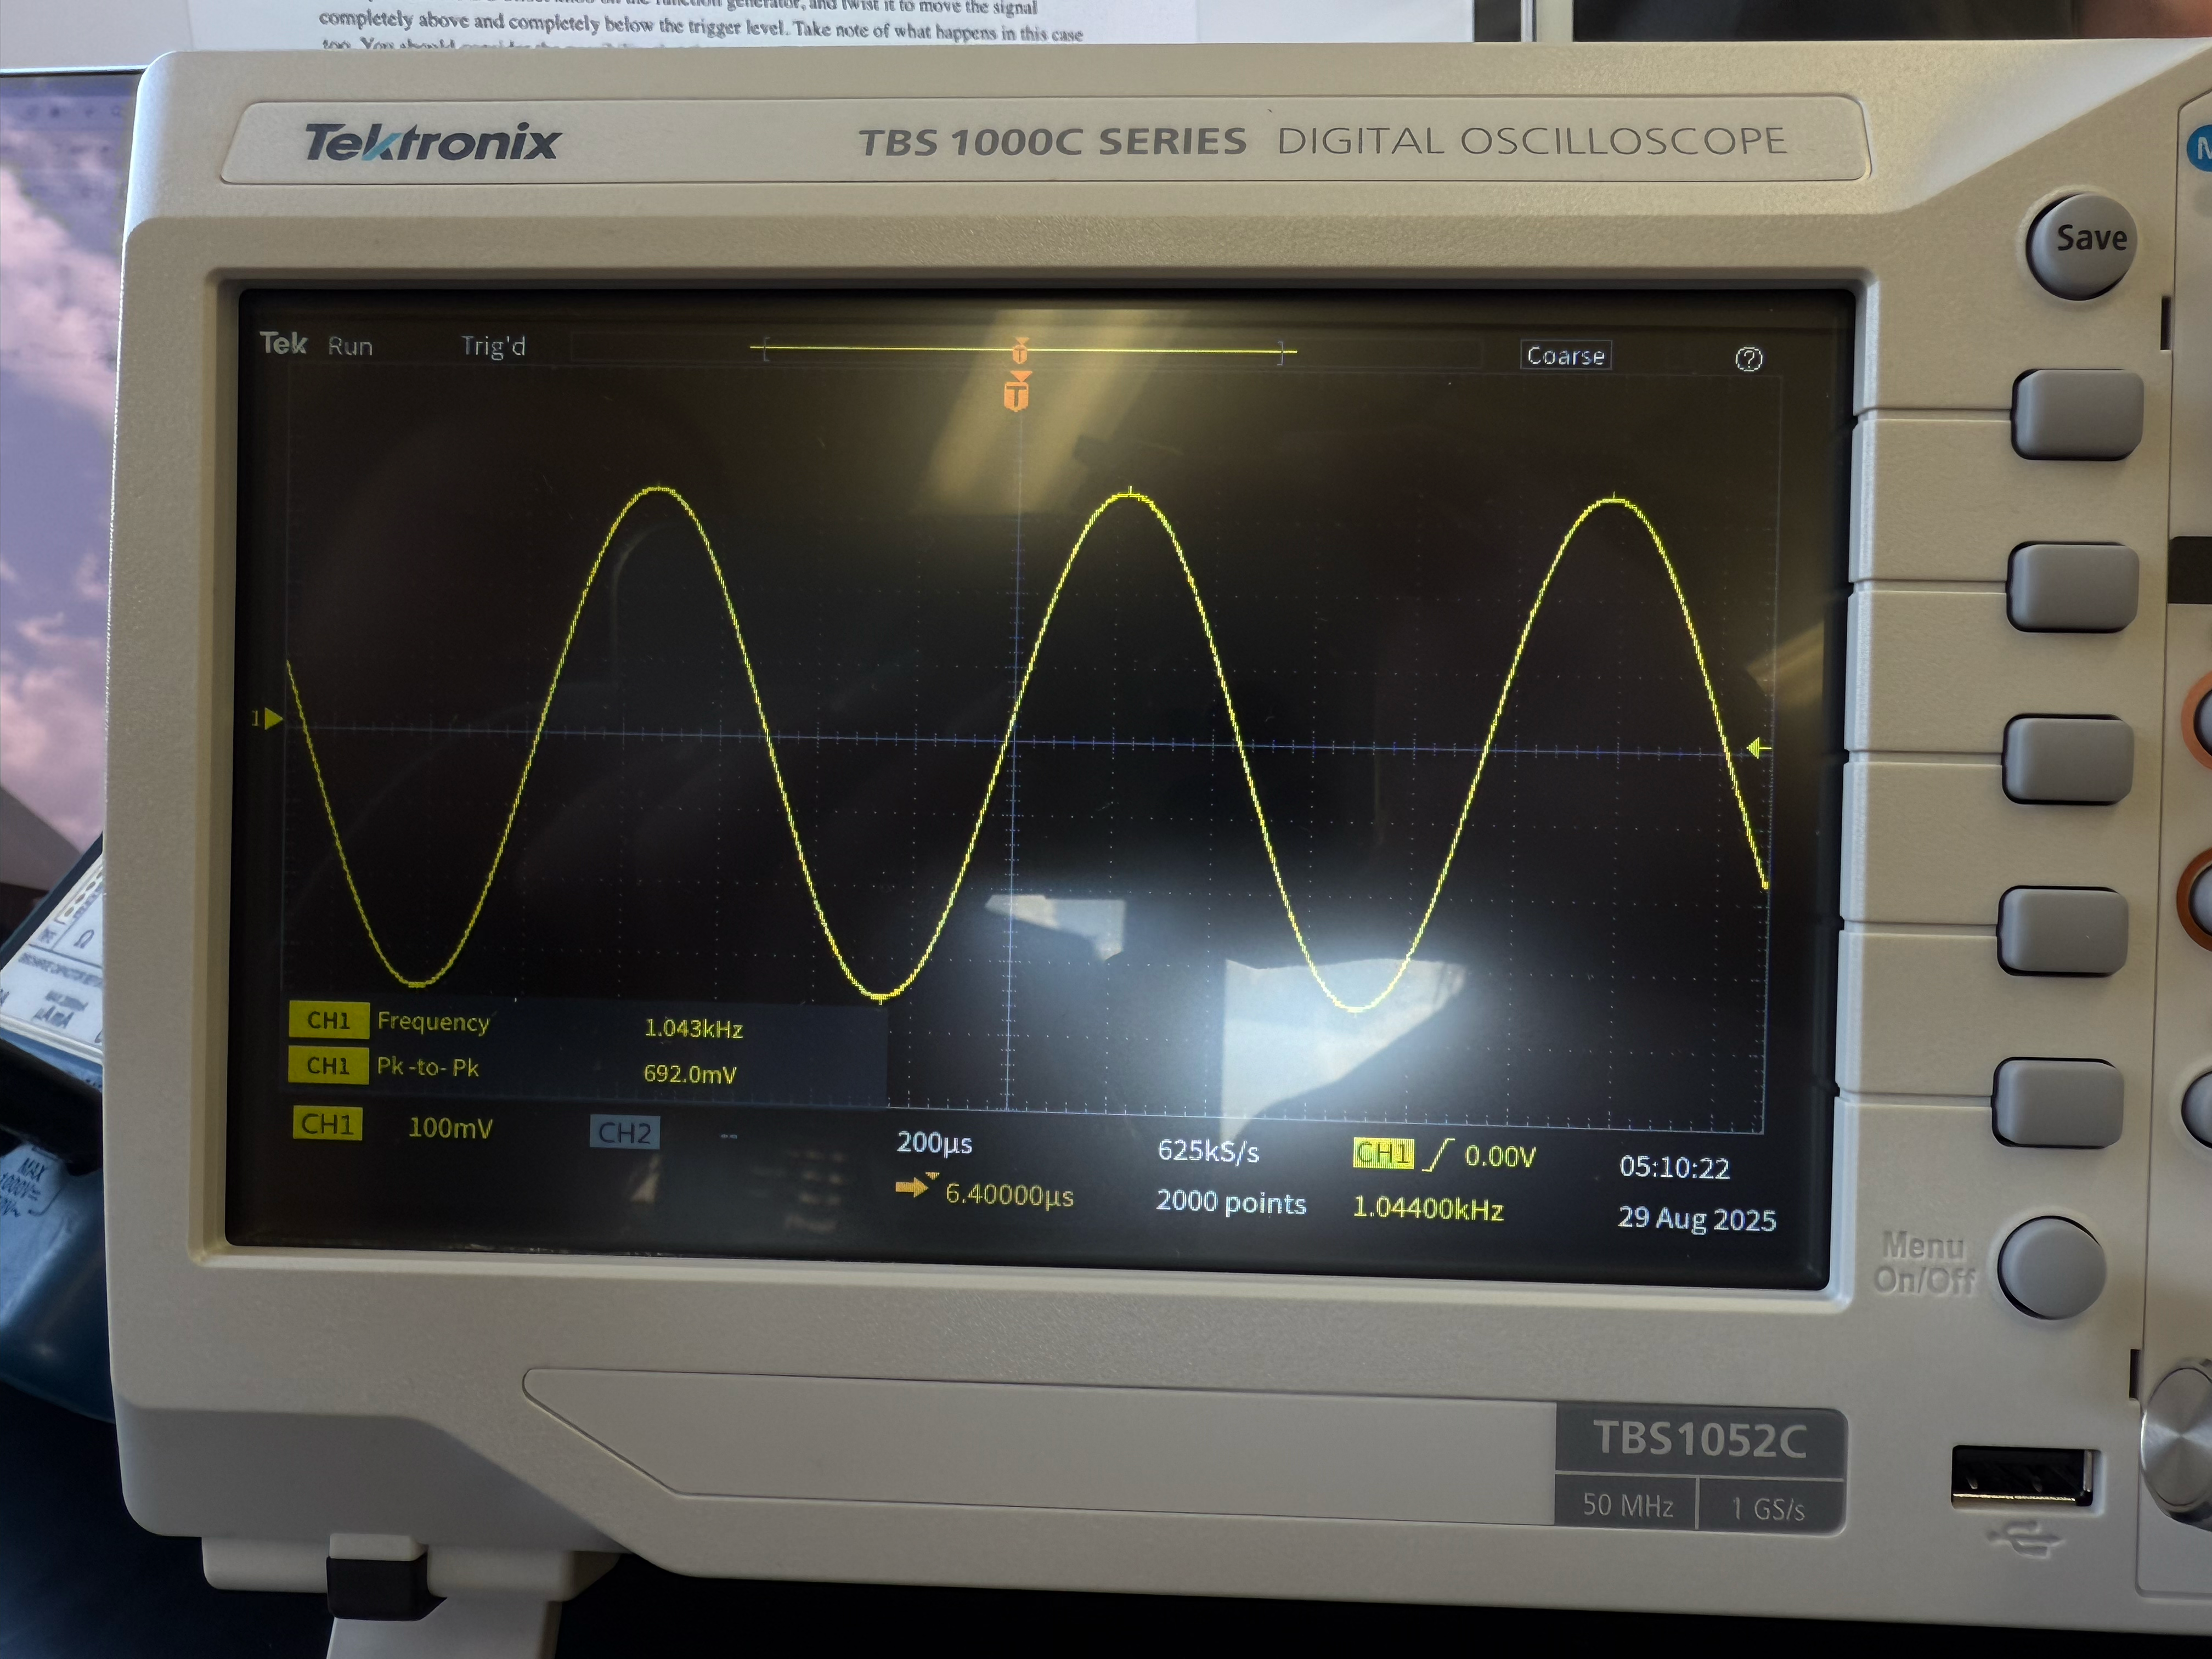
\includegraphics[width=0.47\textwidth]{1.4.aa.png}
    \hfill
    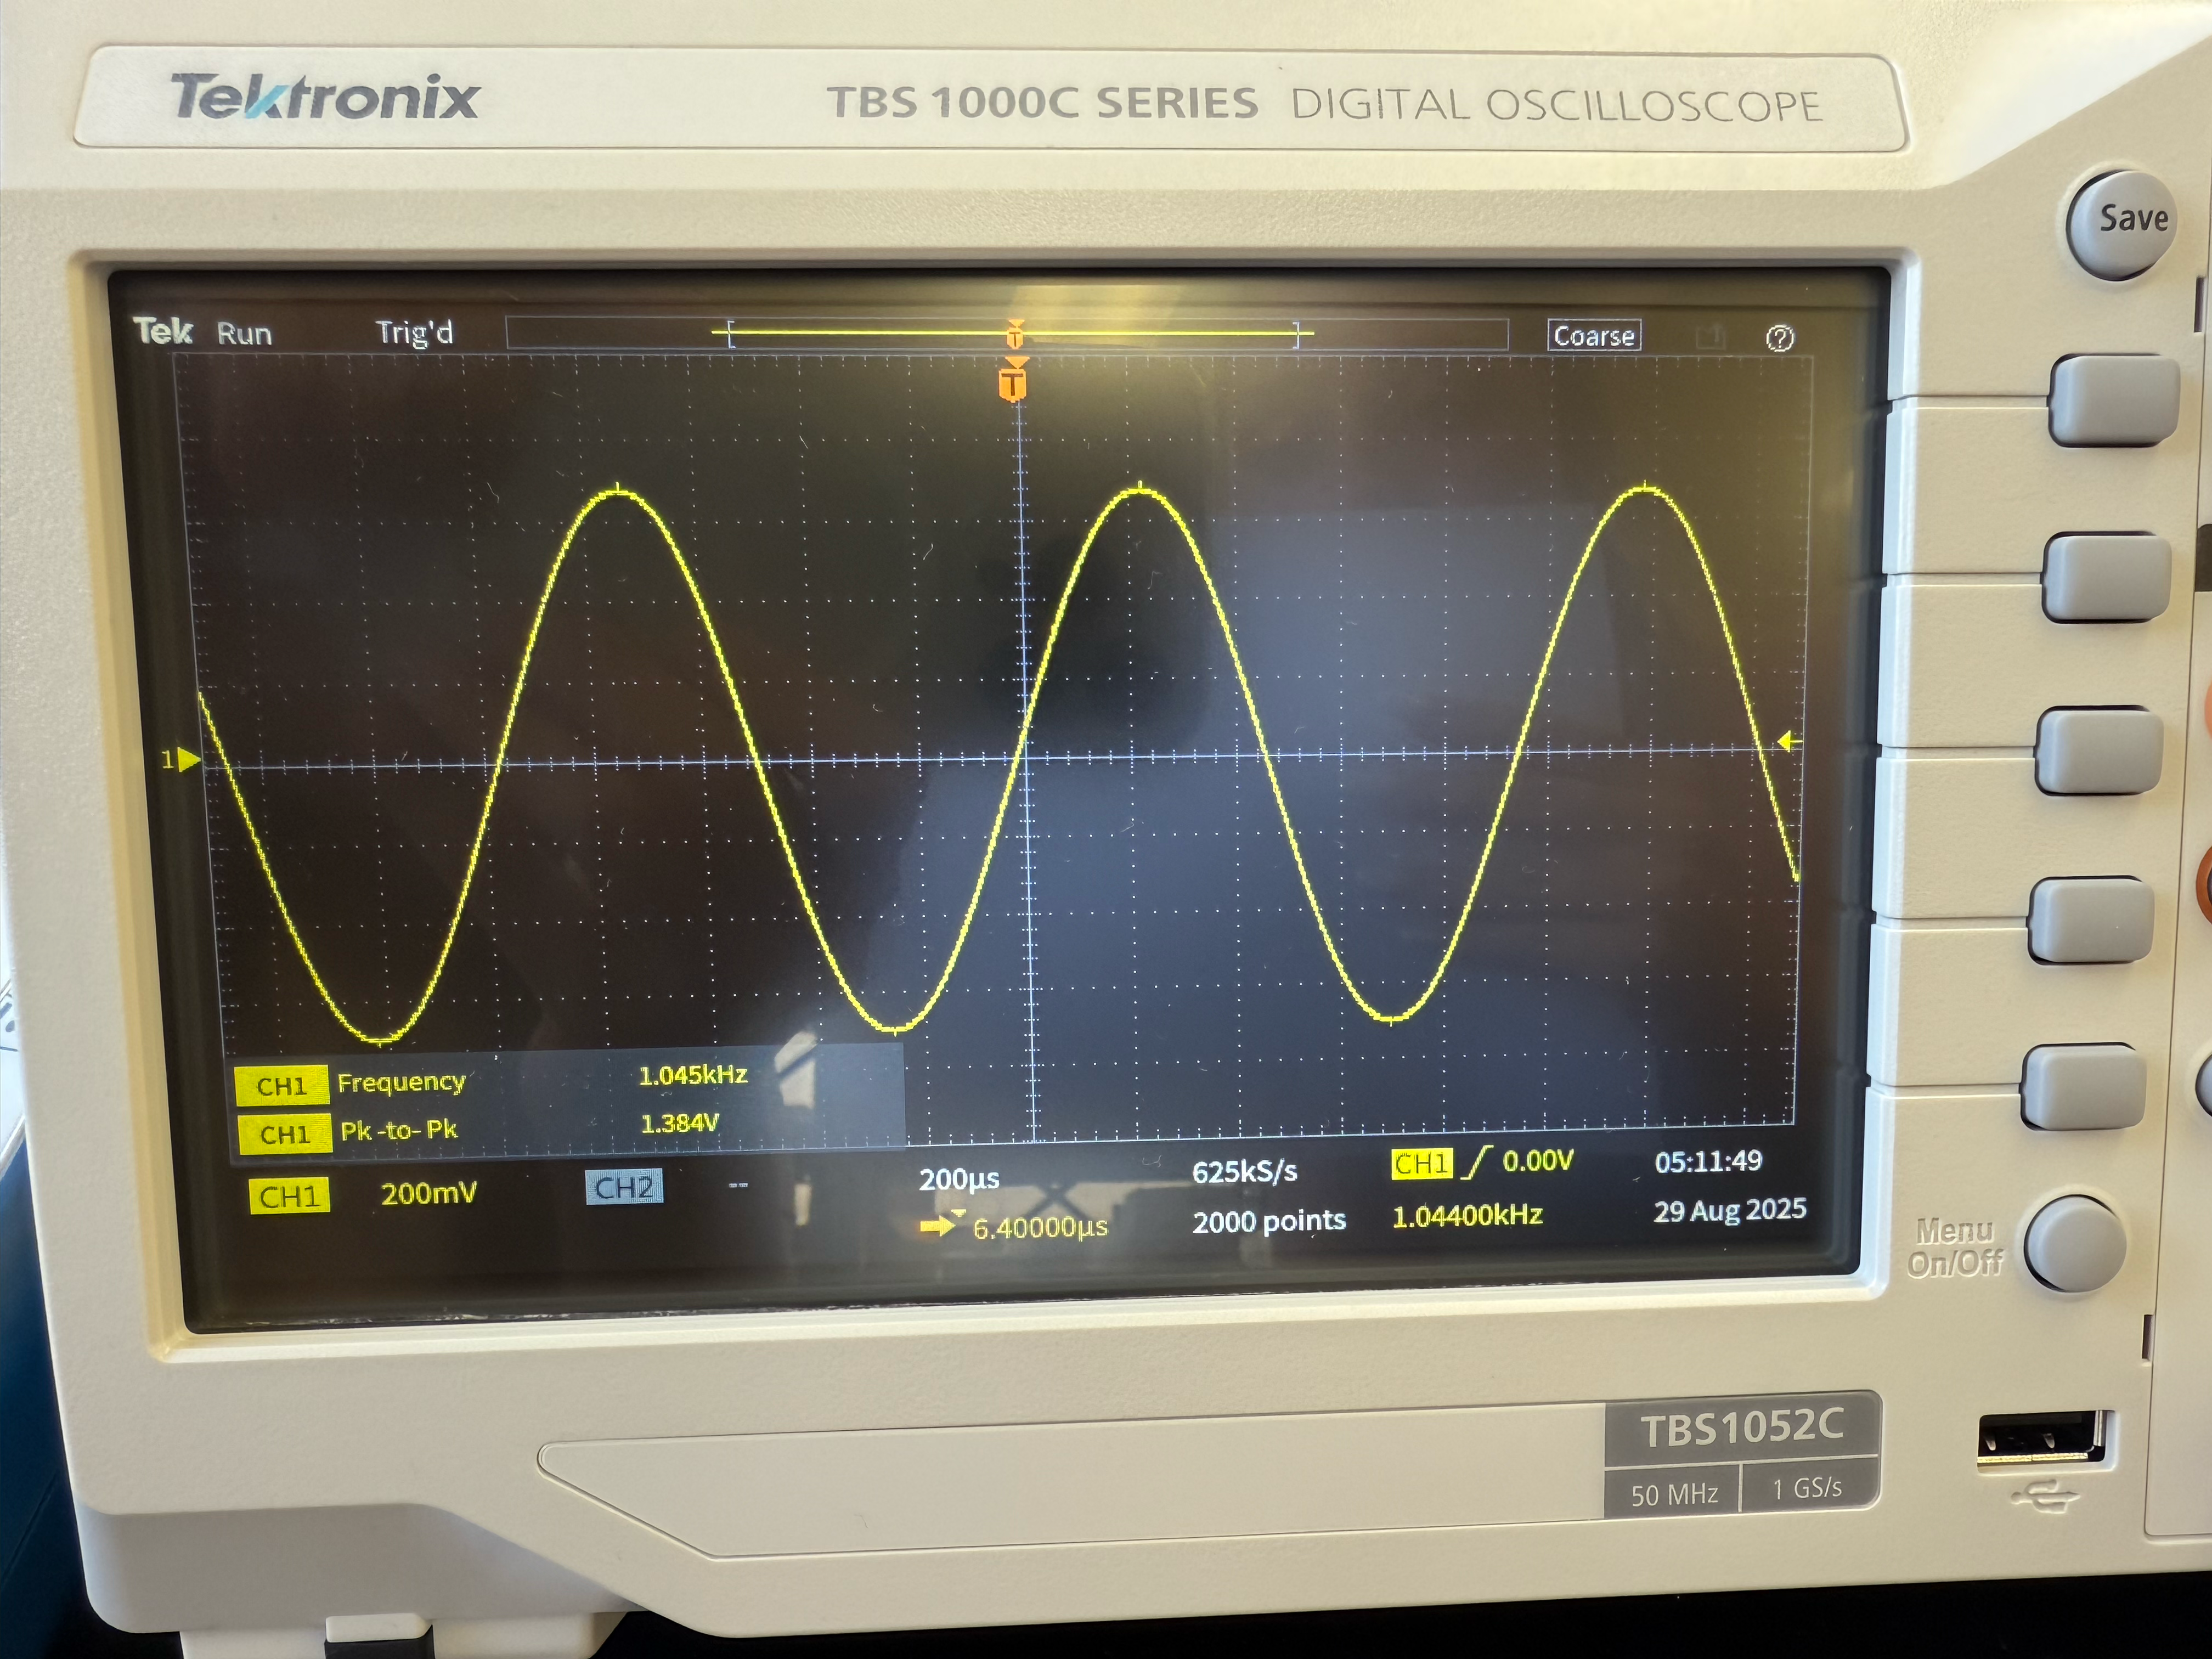
\includegraphics[width=0.47\textwidth]{1.4.ab.png}
    \caption{Oscilloscope display of a 1 kHz sine wave with (left) and without (right) a 50~$\Omega$ terminator.}
    \label{fig:scope_comparison}
\end{figure}

\noindent Without the terminator connected, the oscilloscope's input impedance
(approximately $1\si{\mega\ohm}$) is much larger than the source impedance, so
close to the full open-circuit voltage appears at the input and causes a higher
amplitude. The frequency and shape of the waveform stay constant, which confirms
that the oscilloscope measures voltage rather than current and functions as a
voltmeter, not an ammeter.

\begin{figure}[H]
    \centering
    \includegraphics[width=0.45\textwidth]{1.4.ac.png}
    \hfill
    \includegraphics[width=0.45\textwidth]{1.4.ad.png}
    \caption{Circuit schematics of the function generator and oscilloscope connection with (left) and without (right) a \SI{50}{\ohm} terminator.}
    \label{fig:circuit_comparison}
\end{figure}

\subsubsection{Scope triggering}

When we set the trigger level within the amplitude of the sine wave, the
oscilloscope locked onto a consistent crossing point and displayed a stable
waveform. However, when we moved the trigger level outside the signal's range,
the scope was unable to synchronize to a valid trigger, thus resulting in an
unstable waveform.

\begin{figure}[H]
    \centering
    \includegraphics[width=0.85\textwidth]{1.4.ba.png}
    \caption{Sketch of oscilloscope traces showing a stable sine wave when the trigger level is within the signal range (left) and unstable displays when the trigger level is set above or below the waveform (middle and right).}
    \label{fig:scope_trigger}
\end{figure}

\noindent When we switched the trigger source to the TTL output of the function
generator, the sine remained stable as we adjusted the trigger level up and
down. Even when the DC offset shifted the waveform above or below the trigger
level, the display did not become unstable. The advantage of TTL triggering is
that it provides a well-defined and consistent timing reference that is
independent of the waveform's amplitude or offset.

\begin{figure}[H]
    \centering
    \includegraphics[width=0.60\textwidth]{1.4.bb.png}
    \caption{Sketch of sine wave in CH1 remaining stable when triggered on the TTL output of the function generator (CH2).}
    \label{fig:ttl_output}
\end{figure}

\subsubsection{Square wave}

With DC coupling, changing the DC offset shifted the entire square wave either
up or down relative to ground. With AC coupling, the DC component was blocked 
and the waveform was centered around $0\si{\volt}$ regardless of offset. The
resulting scope display is shown in Figure~\ref{fig:dc_coupling}.

\begin{figure}[H]
    \centering
    \includegraphics[width=0.5\textwidth]{1.4.ca.png}
    \caption{Sketch of oscilloscope display for a square wave with DC offset (shown in DC coupling) and AC coupling.}
    \label{fig:dc_coupling}
\end{figure}

\subsubsection{Function generator output impedance}

We modeled the function generator as a source with an internal resistance
$R_\text{out}$ in series with its output. By attaching different load resistors
$R_\text{Load}$, we measured the corresponding $V_\text{out}$. The circuit
behaves like a voltage divider, described by the equation:

\begin{equation}
    V_\text{out}=V\frac{R_\text{Load}}{R_\text{out}+R_\text{Load}}.
\end{equation}

\noindent Rearranging this into a lienar form gives:

\begin{equation}
    \frac{1}{V_\text{out}}=\frac{1}{V}+\frac{R_\text{out}}{V}\left( \frac{1}{R_\text{Load}}\right)
\end{equation}

\noindent Plotting $1/V_\text{out}$ versus $1/R_\text{Load}$ produced a
straight line, as shown in Figure~\ref{fig:vdiv_plot}. The y-intercept corresponds
to $1/V$, and the slope corresponds to $R_\text{out}/V$. Using these values,
we calculated the open-circuit voltage and the internal output resistance of
the function generator with the formulas:

\begin{align}
    V&=\frac{1}{\text{intercept}}\\
    R_\text{out}&=\frac{\text{slope}}{\text{intercept}}
\end{align}

\begin{figure}[H]
    \centering
    \includegraphics[width=0.8\textwidth]{1.4.d.png}
    \caption{Plot of $1/V_\text{out}$ vs. $1/R_\text{load}$ showing a linear
        relationship consistent with the voltage divider model.}
    \label{fig:vdiv_plot}
\end{figure}

\noindent We used ten load resistors ranging from approximately $50\si{\ohm}$
to $10\si{\kilo\ohm}$. As expected, the $V_\text{out}$ increased with increasing
$R_\text{Load}$, and the plot displayed a clear linear trend consistent with 
theory. The values we extracted, $V=1.99\si{\volt}$ and $R_\text{out}=52.2\si{\ohm}$,
agree within reason with the nominal $50\si{\ohm}$ output impedance of the
function generator. Minor deviations likely came from resistor tolerances, 
cable losses, and oscilloscope measurement error.


\subsubsection{RMS amplitude}

We used a DMM in AC mode to measure the RMS amplitude of sine, triangle, and
square waveforms at $10\si{\hertz}$, $1\si{\kilo\hertz}$, and $100\si{\kilo\hertz}$,
each with a peak-to-peak voltage of $2\si{\volt}$ and zero DC offset. The theoretical
RMS values for a $2V_\text{pp}$ waveform are:

\begin{itemize}
    \item Sine wave: \SI{0.707}{\volt}
    \item Triangle wave: \SI{0.577}{\volt}
    \item Square wave: \SI{1.000}{\volt}
\end{itemize}

\noindent Our measurements are summarized in Table~\ref{tab:rms_measurements} below. At low
frequencies ($10\si{\hertz}$), the DMM significantly under-reported values for
the sine and triangle waves, which is likely due to its limited AC bandwidth
or the internal coupling capacitor not passing low-frequency signals effectively.
At higher frequencies ($10\si{\hertz}$ and $100\si{\kilo\hertz}$), our
measurements approached theoretical values, especially for the square wave.

\begin{table}[H]
    \centering
    \begin{tabular}{ | c c c c | }
        \hline
        Frequency & Sine & Triangle & Square \\
        \hline
        10 Hz   & 0.100 V & 0.120 V & 2.000 V \\
        1 kHz   & 1.980 V & 1.900 V & 2.020 V \\
        100 kHz & 2.060 V & 1.920 V & 2.040 V \\
        \hline
    \end{tabular}
    \caption{Measured RMS amplitudes of sine, triangle, and square waves at different frequencies (2 Vpp input).}
    \label{tab:rms_measurements}
\end{table}

\subsubsection{Rise time}

We set the function generator to produce a $1\si{\mega\hertz}$ square wave and
measured the rise time using the oscilloscope's automatic measurement function. The
rise time, defined as the time it takes for the signal to rise from 10\% to 
90\% of its peak value, was $62.7\si{\nano\second}$. This nonzero value 
reflects the bandwidth of the function generator and oscilloscope, which
constrains how sharply we can reproduce signal transistions.

\begin{figure}[H]
    \centering
    \includegraphics[width=0.5\textwidth]{1.4.f.png}
    \caption{Sketch of observed oscilloscope waveform for a $1\si{\mega\hertz}$ square wave.}
    \label{fig:rise_time}
\end{figure}





\section{Lab 2: RC Circuits}

\subsection{Circuit A}

\subsubsection{Rise and fall time}

Figure~\ref{fig:a_rise_fall} shows the output waveform of Circuit A. We measured 
the time constants for the rising and falling edges as $480\si{\micro\second}$. 
The resistor and capacitor measured with the DMM were $R = 20.11\si{\kilo\ohm}$ and 
$C = 5.48\si{\nano\farad}$, giving a theoretical time constant of $\tau = RC = 110\si{\micro\second}$. 
Thus, the time constant we observed was larger than expected, likely due to 
non-ideal component tolerances and oscilloscope input loading.

\begin{figure}[H]
    \centering
    \includegraphics[width=0.65\linewidth]{2.1.a.png}
    \caption{Output waveform showing the exponential rise and fall of Circuit A.}
    \label{fig:a_rise_fall}
\end{figure}


\subsubsection{Integrator}

Figure~\ref{fig:integrator} shows the output waveforms of Circuit A at various
frequencies. Although we were not able to get a clear square wave shape at the
lowest frequency, as we increased the frequency, the output transitioned to a
more smooth triangular waveform. At low frequncies, the capacitor charged and discharged
more fully, so the output more closely follows the input. At higher frequencies, each
half-cycle becomes shorter, causing the capacitor to charge for less time and reduces
the peak-to-peak amplitude of the output.\\ 

\noindent This behavior is consistent with the expected integrator relation:

\begin{equation}
    V_\text{out}(t) = V_\text{out}(0)+\frac{1}{RC}\int_0^tV_\text{in}(t')\,dt',
\end{equation}

\noindent for $\omega\gg\frac{1}{RC}$, which confirms that Circuit A indeed 
functions as an integrator.

\begin{figure}[H]
    \centering
    \begin{subfigure}[b]{0.45\linewidth}
        \includegraphics[width=\linewidth]{2.1.ba.png}
        \caption{$f = 10.70\si{\kilo\hertz}$}
    \end{subfigure}
    \hfill
    \begin{subfigure}[b]{0.45\linewidth}
        \includegraphics[width=\linewidth]{2.1.bb.png}
        \caption{$f = 15.31\si{\kilo\hertz}$}
    \end{subfigure}
    
    \begin{subfigure}[b]{0.45\linewidth}
        \includegraphics[width=\linewidth]{2.1.bc.png}
        \caption{$f = 22.32\si{\kilo\hertz}$}
    \end{subfigure}
    \hfill
    \begin{subfigure}[b]{0.45\linewidth}
        \includegraphics[width=\linewidth]{2.1.bd.png}
        \caption{$f = 25.82\si{\kilo\hertz}$}
    \end{subfigure}

    \begin{subfigure}[b]{0.45\linewidth}
        \includegraphics[width=\linewidth]{2.1.be.png}
        \caption{$f = 50.04\si{\kilo\hertz}$}
    \end{subfigure}

    \caption{Output voltage of Circuit A at increasing input frequencies.}
    \label{fig:integrator}
\end{figure}


\subsubsection{Low-pass filter}

Next, we tested the frequency response of low-pass filter Circuit A by measuring
the gain and phase shift over a range of frequencies spanning well above and 
below the theoretical cutoff frequency. Figure~\ref{fig:gain_lowpass} shows the gain
plot exhibiting low-pass behavior, with the $3\si{\decibel}$ point occuring near
the expected cutoff frequency of a little over $1\si{\kilo\hertz}$. 
Figure~\ref{fig:phase_lowpass} shows the phase becoming increasingly negative 
with frequency, which aligns with low-pass filter theory.

\begin{figure}[H]
    \centering
    \begin{subfigure}[b]{0.45\linewidth}
        \includegraphics[width=\linewidth]{2.1.ca.png}
        \caption{$f = 12.35\si{\hertz}$}
    \end{subfigure}
    \hfill
    \begin{subfigure}[b]{0.45\linewidth}
        \includegraphics[width=\linewidth]{2.1.cb.png}
        \caption{$f = 1.453\si{\kilo\hertz}$}
    \end{subfigure}

    \begin{subfigure}[b]{0.45\linewidth}
        \includegraphics[width=\linewidth]{2.1.cc.png}
        \caption{$f = 3.492\si{\kilo\hertz}$}
    \end{subfigure}
    \hfill
    \begin{subfigure}[b]{0.45\linewidth}
        \includegraphics[width=\linewidth]{2.1.cd.png}
        \caption{$f = 28.93\si{\kilo\hertz}$}
    \end{subfigure}

    \caption{Representative scope displays for low-pass filter Circuit A at varying frequencies.}
    \label{fig:low_pass}
\end{figure}


\begin{figure}[H]
    \centering
    \includegraphics[width=0.65\textwidth]{2.1.cgain.png}
    \caption{Gain vs. frequency for the low-pass filter Circuit A.}
    \label{fig:gain_lowpass}
\end{figure}


\begin{figure}[H]
    \centering
    \includegraphics[width=0.65\textwidth]{2.1.cphase.png}
    \caption{Phase shift vs. frequency for the low-pass filter..}
    \label{fig:phase_lowpass}
\end{figure}



\subsection{Circuit B}

\subsubsection{Time constants}

We drove circuit B with a square wave (no DC offset) to observe exponential
decays during each transition. A copy of the waveform is shown in Figure~\ref{fig:b_time_constants}.

\begin{figure}[H]
    \centering
    \includegraphics[width=0.65\linewidth]{2.2.a.png}
    \caption{Output waveform showing the the exponential decays for Circuit B.}
    \label{fig:b_time_constants}
\end{figure}

\noindent From the oscilloscope, we measured the positive
decay time constant as $340\si{\micro\second}$ and the negative time decay
constant as $444\si{\micro\second}$. The measurements differ slightly, which
is likely due to measurement error or asymmetries in the circuit. The theoretical
time constant is $\tau = RC = 110\si{\micro\second}$. Our measurements 
were higher but within the same order of magnitude than the predicted value, which
may result from input loading or limitations in cursor placement on the oscilloscope.



\subsubsection{Differentiator}

We configured Circuit B as a differentiator and applied a triangle wave input
at various frequencies. According to Equation (2.2):

\begin{equation}
    V_\text{out}=RC\frac{dV_\text{in}}{dt},
\end{equation}

\noindent the output should approximate the derivative of the input waveform when the
driving frequency satisfies $\omega << \frac{1}{RC}$.\\

\noindent As shown in Figure~\ref{fig:diff}, at high frequencies,
the output follows the triangular input, which indicates the circuit is
not acting as a differentiator. As we decreased the frequency, the waveform
started to resemble a square wave, which is the expected derivative of a triangle wave
since triangle slopes are constant. The lowest frequency we tested was $196.9\si{\hertz}$.
At this value, the output approximates an ideal square wave, which confirms 
expected differentiator behavior.

\begin{figure}[H]
    \centering
    \begin{subfigure}[b]{0.32\textwidth}
        \includegraphics[width=\textwidth]{2.2.bb.png}
        \caption{10.11 kHz}
    \end{subfigure}
    \hfill
    \begin{subfigure}[b]{0.32\textwidth}
        \includegraphics[width=\textwidth]{2.2.bd.png}
        \caption{6.883 kHz}
    \end{subfigure}
    \hfill
    \begin{subfigure}[b]{0.32\textwidth}
        \includegraphics[width=\textwidth]{2.2.bc.png}
        \caption{4.425 kHz}
    \end{subfigure}
    
    \vspace{0.5em}
    
    \begin{subfigure}[b]{0.32\textwidth}
        \includegraphics[width=\textwidth]{2.2.be.png}
        \caption{1.145 kHz}
    \end{subfigure}
    \begin{subfigure}[b]{0.32\textwidth}
        \includegraphics[width=\textwidth]{2.2.bf.png}
        \caption{196.9 Hz}
    \end{subfigure}
    
    \caption{Output waveforms of the RC differentiator circuit at various input triangle wave frequencies.}
    \label{fig:diff}
\end{figure}



\subsubsection{High-pass filter}

Next, we measured the gain and phase of high-pass filter Circuit B 
as a function of frequency. Scope traces at four different frequencies are
included in Figure~\ref{fig:high_pass_scope}, showing how the output
signal evolves along with frequency.

\begin{figure}[H]
    \centering
    \begin{subfigure}[b]{0.45\textwidth}
        \includegraphics[width=\textwidth]{2.2.ca.png}
        \caption{52.5 kHz}
    \end{subfigure}
    \hfill
    \begin{subfigure}[b]{0.45\textwidth}
        \includegraphics[width=\textwidth]{2.2.cb.png}
        \caption{8.7 kHz}
    \end{subfigure}
    \begin{subfigure}[b]{0.45\textwidth}
        \includegraphics[width=\textwidth]{2.2.cc.png}
        \caption{996 Hz}
    \end{subfigure}
    \hfill
    \begin{subfigure}[b]{0.45\textwidth}
        \includegraphics[width=\textwidth]{2.2.cd.png}
        \caption{116 Hz}
    \end{subfigure}
    \caption{Oscilloscope displays of input (CH1) and output (CH2) voltages for the high-pass filter at various drive frequencies.}
    \label{fig:high_pass_scope}
\end{figure}

\noindent The gain curve in figure ~\ref{fig:gain_highpass} shows that the
filter passes high frequencies while suppressing low ones, as expected. The $3\si{\decibel}$
point occurs at a little over $1\si{\kilo\hertz}$ and marks the cutoff frequency. The 
phase shift plot in Figure~\ref{fig:phase_highpass} shows the transistion from $90^\circ$
to $0^\circ$ at higher frequencies. This behavior is consistent with what
is expected with a first-order high-pass filter.

\begin{figure}[H]
    \centering
    \includegraphics[width=0.65\textwidth]{2.2.cgain.png}
    \caption{Gain vs. frequency for the high-pass filter.}
    \label{fig:gain_highpass}
\end{figure}

\begin{figure}[H]
    \centering
    \includegraphics[width=0.65\textwidth]{2.2.cphase.png}
    \caption{Phase shift vs. frequency for the high-pass filter.}
    \label{fig:phase_highpass}
\end{figure}


\subsection{Comparison with theory}

\subsubsection{Circuit A}

To analyze the low-pass circuit A, we used the complex impedance method to
derive the gain and phase shift as functions of frequency. The transfer
function is:
\begin{equation}
    \frac{V_\text{out}}{V_\text{in}}=\frac{1}{1+j\omega RC}.
\end{equation}

\noindent Taking the magnitude gives us the theoretical gain:
\begin{equation}
    \left|\frac{V_\text{out}}{V_\text{in}}\right|=\frac{1}{\sqrt{1+(\omega RC)^2}},
\end{equation}

\noindent which makes the phase shift:
\begin{equation}
    \phi=-\arctan(\omega RC).
\end{equation}

\noindent Using the values $R=20\si{\kilo\ohm}$ and $C=0.005\si{\micro\farad}$, 
we plotted the theoretical gain and phase shift versus frequency. The cutoff
occurs at $f_0=\frac{1}{2\pi RC}\approx 1.6\si{\kilo\hertz}$ where the gain drops
to $0.707$, which is the $-3\si{\decibel}$ point. The phase shift transistions
from $0^\circ$ at low frequencies to $-90^\circ$ at high frequencies.

\begin{figure}[H]
    \centering
    \begin{subfigure}[b]{0.48\textwidth}
        \centering
        \includegraphics[width=\textwidth]{2.3.a.gain.png}
        \caption{Ideal gain vs. frequency.}
        \label{fig:a_theory_gain}
    \end{subfigure}
    \hfill
    \begin{subfigure}[b]{0.48\textwidth}
        \centering
        \includegraphics[width=\textwidth]{2.3.a.phase.png}
        \caption{Ideal phase shift vs. frequency.}
        \label{fig:a_theory_phase}
    \end{subfigure}
    \caption{Theoretical frequency responses for Circuit A (low-pass filter).}
    \label{fig:a_theory}
\end{figure}

\noindent Our measured gain and phase data align well with the theory
across most of the frequency range, which confirms the expected behavior of a
low-pass filter. Minor discrepancies appear at higher frequencies (above 20kHz),
where the gain decreases more rapidly and the phase shift begins to flatten.
These likely reflect non-ideal effects such capacitor ESR or parasitic
inductance, which become more pronounced at high frequencies. Overall.


\subsubsection{Circuit B}

To analyze the high-pass Circuit B, we used the complex impedance method to 
derive the gain and phase shift as functions of frequency. The transfer 
function is: 
\begin{equation}
\frac{V_\text{out}}{V_\text{in}} = \frac{j\omega RC}{1 + j\omega RC}.
\end{equation}

\noindent Taking the magnitude gives us the theoretical gain:
\begin{equation}
\left|\frac{V_\text{out}}{V_\text{in}}\right| = \frac{\omega RC}{\sqrt{1 + (\omega RC)^2}}.
\end{equation}

\noindent which makes the phase shift:
\begin{equation}
\phi = 90^\circ-\arctan(\omega RC).
\end{equation}

\begin{figure}[H]
    \centering
    \begin{subfigure}[b]{0.48\textwidth}
        \centering
        \includegraphics[width=\linewidth]{2.3.b.gain.png}
        \caption{Ideal gain vs. phase shift.}
        \label{fig:highpass_gain}
    \end{subfigure}
    \hfill
    \begin{subfigure}[b]{0.48\textwidth}
        \centering
        \includegraphics[width=\linewidth]{2.3.b.phase.png}
        \caption{Ideal phase shift vs. frequency.}
        \label{fig:highpass_phase}
    \end{subfigure}
    \caption{Theoretical frequency responses for Circuit B (high-pass filter).}
    \label{fig:circuitB_theory}
\end{figure}


\noindent Our theoretical plots of gain and phase versus frequency confirm
the expected high-pass filter behavior where gain approaches zero at low
frequencies and approaches 1 at high frequencies. The phase starts near $-90^\circ$
and approaches $0^\circ$ as frequency increases.\\

\noindent Our measured data agrees with the theoretical models. The
$3\si{\decibel}$ point occurs at the cutoff frequency ($\approx 1.6\si{\kilo\hertz}$),
and both plots generally follow the predicted trend, though we observed minor
deviations due to experimental noise or oscilloscope resolution limits. Overall,
our measurements confirm the behavior of an ideal high-pass filter. 



\section{Lab 3: Inductors and LC Filter Circuits}

\subsection{Impedance measurement with the LCR meter}

We used a Bourns RL181S-102J-RC inductor to observe how its impedance 
characteristics change with frequency. We measured the inductor's properties 
at four different frequencies (\SI{100}{\hertz}, \SI{1}{\kilo\hertz}, \SI{10}{\kilo\hertz}, 
and \SI{100}{\kilo\hertz}) using an LCR meter. We obtained the series inductance $L_S$, 
quality factor $Q$, equivalent series resistance (ESR), and phase angle $\theta$. The 
results are summarized in Table~\ref{tab:bourns_table}.

\begin{table}[H]
    \centering
    \begin{tabular}{|c|c|c|c|c|}
    \hline
    \text{Frequency} & $L_S$ (µH) & $Q$ & \text{ESR (Ω)} & $\theta$ (deg) \\
    \hline
    100 Hz   & 950.0   & 0.274  & 2.1   & 15.3  \\
    1 kHz    & 944.4   & 2.69   & 2.2   & 69.6  \\
    10 kHz   & 944.6   & 23.7   & 2.5   & 87.5   \\
    100 kHz  & 928.5   & 137.0  & 4.12  & 89.5  \\
    \hline
    \end{tabular}
    \caption{Measured inductor parameters (Bourns RL181S-102J-RC) at various frequencies.}
    \label{tab:bourns_table}
\end{table}

\noindent According to the manufacturer’s datasheet, the inductor has a nominal 
inductance of \SI{1000}{\micro\henry} with a tolerance of $\pm 5\%$, a minimum 
quality factor $Q = 70$ at \SI{50}{\kilo\hertz}, and a self-resonant 
frequency (SRF) of \SI{0.77}{\mega\hertz}. Our measured inductance values 
ranged from \SI{928.5}{\micro\henry} to \SI{950.0}{\micro\henry}, which are 
well within our expectations.\\

\noindent From our measurements, we observed that at low frequencies 
(\SI{100}{\hertz}), the inductor deviated significantly from ideal behavior, 
exhibiting a low quality factor ($Q$) and a small phase angle ($\theta$). As 
the frequency increased, the inductor's behavior approached that of an ideal 
inductor. $Q$ increased, $\theta$ approached \SI{90}{\degree}, and the ESR 
remained relatively low. The inductor behaved most ideally between \SI{10}{\kilo\hertz} 
and \SI{100}{\kilo\hertz}, where $Q$ was high and the phase angle was nearly \SI{90}{\degree}.\\

\noindent To verify the consistency of ESR and $Q$ values, we used the 
definition of quality factor:
\begin{equation}
    Q=\frac{\omega L_s}{\text{ESR}}.
\end{equation}

\noindent At $f=$\SI{1}{\kilo\hertz}, using $L_S = \SI{944.4}{\micro\henry}$ 
and ESR = \SI{2.2}{\ohm}, we computed:

\begin{equation}
    Q=\frac{2\pi(1000)(944.4\times 10^{-6})}{2.2}\approx 2.70,
\end{equation}

\noindent which indeed matches the measured value of $Q = 2.69$ and confirms 
the consistency of our data.\\

\noindent We also measured the impedance characteristics of a \SI{100}{\nano\farad} 
ceramic capacitor using the same LCR meter across the same set of frequencies. The 
results are summarized in Table~\ref{tab:capacitor_table}.

\begin{table}[H]
    \centering
    \begin{tabular}{|c|c|c|c|c|}
    \hline
    \text{Frequency} & $C_S$ (nF) & $D$ & \text{ESR (Ω)} & $\theta$ (deg) \\
    \hline
    100 Hz   & 99.37  & 0.000 & n/a   & -90.0 \\
    1 kHz    & 99.33  & 0.000 & 0.20  & -90.0 \\
    10 kHz   & 99.28  & 0.000 & 0.06  & -90.0 \\
    100 kHz  & 99.31  & 0.001 & 0.02  & -90.0 \\
    \hline
    \end{tabular}
    \caption{Measured parameters for 100nF ceramic capacitor at various frequencies.}
    \label{tab:capacitor_table}
\end{table}

\noindent Across all frequencies, the measured capacitance remained  
consistent around \SI{99.3}{\nano\farad}. The phase angle $\theta$ also stayed consistently at \SI{-90}{\degree}, suggesting nearly ideal capacitive behavior. The dissipation factor $D$ remained extremely low and the equivalent series resistance (ESR) decreased with increasing frequency, which is what we expected.\\

\noindent Comparing both components, the ceramic capacitor exhibited behavior 
much closer to an ideal capacitor than the inductor did to an ideal inductor. 
Its phase angle stayed the same at \SI{-90}{\degree} and the ESR was minimal 
across the entire frequency range. The dissipation factor $D$ being close to $0$ 
also indicates that nearly all the energy is stored and returned rather than 
dissipated as heat. The inductor, on the other hand, only approached ideal 
behavior at higher frequencies (\SI{10}{\kilo\hertz} and above).



\subsection{Impedance measurements with an oscilloscope}
 
We used the oscilloscope to measure the voltage across the inductor (CH1), 
the voltage across the series resistor (MATH), and the phase difference 
between them. Although we intended to measure at $1\si{\kilo\hertz}$, the
signal generator was inadvertently set to $25.42\si{\kilo\hertz}$ and the
waveform somewhat unstable. We performed our analysis based on this actual
frequency.

\begin{figure}[H]
    \centering
    \includegraphics[width=0.65\textwidth]{3.b.png}
    \caption{Oscilloscope display showing voltage across the inductor (CH1), 
    voltage across the resistor(MATH).}
    \label{fig:scope_inductor}
\end{figure}

\noindent The voltage across the inductor was $496\si{\milli\volt}$, and the voltage
across the resistor was $1.00\si{\volt}$, giving us a current of $10\si{\milli\ampere}$.
Using the relation $L_S = V_L/ (\omega I)$ and $\omega=2\pi f=159719\si{\radian} / \si{\second}$,
we calculated:
\begin{equation}
    L_S = \frac{0.496}{159719\cdot 0.01}\approx 311\si{\micro\henry}.
\end{equation}

\noindent This value is significantly lower than the LCR measurement at $1\si{\kilo\hertz}$
($944\si{\micro\henry}$), likely due to frequency dependence and limitations in
the CH1 measurement. We calculated the ESR as $V_R / I=100\si{\ohm}$ and the quality
factor as:
\begin{equation}
    Q=\frac{\omega L_S}{\text{ESR}}\approx 0.50.
\end{equation}

\noindent We estimated the phase angle visually using the oscilloscope and approximated
the time offset between the CH1 and MATH waveforms as $7.1\si{\micro\second}$.
With a waveform period of $T=1/f\approx 39.3\si{\micro\second}$, this
corresponds to:
\begin{equation}
    \theta \approx 360^\circ \cdot \frac{7.1}{39.3}\approx 64^\circ.
\end{equation}

\noindent The current we measured of $10\si{\milli\ampere}$ is well below the rated
maximum of $90\si{\milli\ampere}$, which confirms the component was not
approaching saturation or overheating during measurement.\\

\noindent Finally, we went through input frequencies from $50\si{\kilo\hertz}$ to
$1\si{\mega\hertz}$ and observed resonance behavior near $770\si{\kilo\hertz}$.
This agrees with the inductor's specified SRF of $0.77\si{\mega\hertz}$. Beyond
this point, the inductor exhibits capacitive behavior.


\subsection{Notch filter}

\noindent Next, we built a notch filter RLC circuit using a $1\si{\milli\henry}$ inductor
and a $4.7\si{\nano\farad}$ capacitor. We measured the gain $|\widetilde{V}_\text{out} / \widetilde{V}_\text{in}|$
across a range of frequencies and plotted it in Figure~\ref{fig:notch_gain}.
As expected for a series notch filter, the gain goes through a sharp dip near
the resonant frequency since this is where the voltage drops due to impedance
cancellation between the inductor and capacitor.

\begin{figure}[H]
    \centering
    \includegraphics[width=0.6\textwidth]{3.ca.png}
    \caption{Gain vs. frequency for the notch filter circuit.}
    \label{fig:notch_gain}
\end{figure}

\noindent From the plot, we observed the minimum gain occurs at approximately $f_0\approx 73.2\si{\kilo\hertz}$,
where $|\widetilde{V}_\text{out} / \widetilde{V}_\text{in}|\approx 0.084$. We visually
estimated the $-3\si{\decibel}$ points to be $68\si{\kilo\hertz}$ and $81\si{\kilo\hertz}$,
giving us a bandwidth of approximately $13.0\si{\kilo\hertz}$. We calculated the experimental
quality factor:
\begin{equation}
    Q=\frac{f_0}{\text{bandwidth}}=\frac{73.2\si{\kilo\hertz}}{13.0\si{\kilo\hertz}}\approx 5.63.
\end{equation}

\noindent Next, we find the equivalent series resistance to reach this quality factor:
\begin{equation}
    R=\frac{1}{Q} \sqrt{\frac{L}{C}} \approx 81.9\si{\ohm}.
\end{equation}

\noindent This value corresponds to the total resistance in the inductor and circuit wiring.
The relatively sharp notch and moderate $Q$ suggest reasonable energy loss and 
confirm the expected series RLC behavior.\\

\noindent Our theoretical predictions also align with our measured values. 
Using $L = 1\si{\milli\henry}$ and $C = 4.7\si{\nano\farad}$, we calculate the 
resonant frequency:
\begin{equation}
    f_0 = \frac{1}{2\pi\sqrt{LC}} \approx 73.3\si{\kilo\hertz},
\end{equation}
which is close to our observed value of $f_0 \approx 73.2\si{\kilo\hertz}$. 
Thus, we confirm our notch filter setup behaves as expected in theory.


\subsection{Second-order Butterworth filter}

Finally, we constructed a second-order Butterworth filter using a $1\si{\milli\henry}$
inductor and a $4.47\si{\nano\farad}$ capacitor, which gives us a resonant
(cuttoff) frequency of approximately $73.3\si{\kilo\hertz}$. From the formula
for an ideal Butterworth filter:
\begin{equation}
    R=\frac{1}{2\sqrt{2}\pi f_0 C},
\end{equation}

\noindent we found the required resistor value to be about $343.5\si{\ohm}$. We used three $100\si{\ohm}$
resistors in series to give us a total resistance of roughly $300\si{\ohm}$ during our experiment.\\

\noindent We measured $|\widetilde{V}_\text{out} / \widetilde{V}_\text{in}|$ at various frequencies
and plotted the our data on a log-log scale. The curve shows the gain close to $1$
at low frequencies, then begins to decrease beyond the resonant (cutoff) frequency,
which is expected behavior of a second-order Butterworth filter.\\

\noindent At high frequencies, the gain should fall off as $1/f^2$, which corresponds to
a slope of $-40\si{\decibel}$ per order in a log-log plot. Our data generally follows
the expected slope in the high-frequency region, which confirms that our filter
behaves as predicted. Minor deviations are likely due to component tolerances
or limitations in the measurement setup.

\begin{figure}[H]
    \centering
    \includegraphics[width=0.6\textwidth]{3.da.png}
    \caption{Gain vs. frequency on a log-log scale for the second-order Butterworth filter.}
    \label{fig:butterworth_gain}
\end{figure}

\section*{Acknowledgements}

We would like to thank our laboratory instructor, Dr. Heinzen, and our teaching 
assistant, Kyle Gable, for their guidance and support through these labs. Their 
assistance and feedback were invaluable in helping us understand the experimental 
procedures and circuit concepts. We also appreciate the department's laboratory 
facilities and equipment, which made these experiments possible.

\end{document}